\documentclass[12pt]{article}

\usepackage[margin=2cm]{geometry}
\usepackage{amsmath}
\usepackage{multicol}
\usepackage{nopageno}
\usepackage{SIunits}
\usepackage{graphicx}
\usepackage{enumerate}
\usepackage{enumitem}
%\usepackage{mathabx}
\usepackage{wasysym}


% for making bond drawings
\usepackage{chemfig}
% Global bond settings
\setchemfig{
  atom sep=18pt,               % fixed bond length
  double bond sep=2pt,       % spacing between the two bars
  bond style={line width=0.8pt}
}


% for centering figures on page while in an enumerated/itemized list:
\usepackage{changepage} % in the preamble
\makeatletter
\newenvironment{centerinpage}
  {%
    \par\noindent
    \hspace*{-\@totalleftmargin}% back to page margin (covers all nested list indents)
    \begin{minipage}{\textwidth}% fixed to page width (ignores widened \linewidth)
      \centering
  }
  {%
    \end{minipage}\par
  }
\makeatother

%%%%%%%%%%%%%%%%%%%%%%%%%%%%%%%%%%%%%%%%%%%%%%%%%%%%%
% For putting links in the document (both to sections and hyperlinks)
\usepackage{hyperref}
\usepackage{url}
\hypersetup{
    colorlinks=true,     % false: boxed links; true: colored links
    linkcolor=red,       % color of internal links
    citecolor=blue,      % color of links to bibliography
    filecolor=blue,      % color of file links
    urlcolor=blue        % color of external links
}
% below, use \url{http://www.nytimes.com} (they will be urlcolor)
%%%%%%%%%%%%%%%%%%%%%%%%%%%%%%%%%%%%%%%%%%%%%%%%%%%%%


%%%%%%%%%%%%%%%%%%%%%%%%%%%%%%%%%%%%%%%%%%%%%%%%%%%%%
% for the events page boxes

% boxed regions
\usepackage{tcolorbox}
\tcbuselibrary{skins,breakable}

% fonts & spacing
\usepackage{lmodern}
\usepackage{microtype}
\usepackage{calc}


% small helper macros (adjust these)
\newcommand{\boxheight}{4.2cm}   % height for each event box
\newcommand{\boxfont}{\scriptsize} % change to \tiny or \footnotesize as desired
\newcommand{\linelen}{0.95\linewidth} % timeline line length

%%%%%%%%%%%%%%%%%%%%%%%%%%%%%%%%%%%%%%%%%%%%%%%%%%%%%
\newcommand{\rmd}{\ensuremath{{\rm d}}}
%\newcommand{\vv}[1]{\ensuremath{\vec{#1}}}
\newcommand{\vv}[1]{\ensuremath{\mathbf{#1}}}
\newcommand{\ee}[1]{\ensuremath{\mathbf{e}_{#1}}}
%%%%%%%%%%%%%%%%%%%%%%%%%%%%%%%%%%%%%%%%%%%%%%%%%%%%%



\begin{document}

\begin{center}
{\Large Greenhouse Effect: Matter and Light Interaction (two days)}
\end{center}

\noindent Here we'll focus on a single topic: how light interacts with molecules to produce the greenhouse effect.  This will require us to first review (i) basic physics concepts of electric charges, forces, and fields; and (ii) the basic chemistry concepts (ultimately arising from {\em quantum} physics) of atoms, bonding, and molecule geometry.  We will then put the two together under the basic rule:
	%
	\begin{quote}
	 {\em Infrared photons can be captured by a molecule if that molecule's net electric dipole can be changed by the photon's electric field.} These changes to the dipole will occur concurrently with (because of) vibrations or rotations of the molecules, which is where the energy of the photon goes when captured.
	\end{quote}
	%
Let's jump right to the point with some example applications of the rule for atmospheric gases:
	%
	\begin{itemize}
	\item {\bf Nitrogen}  ($\text{N}_2$; \chemfig{N~N}; 78\% of the ``dry'' atmosphere) and {\bf Oxygen} ($\text{O}_2$, \chemfig{O=O}, 21\% of the atmosphere)  are each perfectly symmetric linear diatomic molecules. That symmetry is maintained under vibration (stretching and contracting). Therefore they have always have zero net electric dipole.  Therefore their dipole moment is unchanging regardless of a photon's electric field. Therefore they do not capture (infrared) photons.  This means that 99\% of the gases in the (dry) atmosphere are {\em not} greenhouse gases!
	\item {\bf Carbon Dioxide} ($\text{C}\text{O}_2$; \chemfig{O=C=O}; $\unit{425}{ppm} = 425 / 10^6 = 0.000425 = 0.0425 \%$ of the atmosphere) is a symmetric linear molecule.  One can imagine two internal electric dipoles pointing along the bonds from C to each O, but these vectors point in opposite directions and sum to a net dipole of zero.  If the molecule stretches symmetrically (keeping the two bond lengths equal) then the net dipole moment remains zero (two longer, but still opposite, vectors sum to zero). However, if one \chemfig{C=O} bond is stretched more than the other, then there {\em will} be a net dipole.  So infrared photons can be captured to cause that type of (asymmetric) vibration.  Additionally: if the molecule {\em bends}, the net dipole will be nonzero; therefore it can absorb infrared photons to induce bending oscillations.  Carbon dioxide is a greenhouse gas.
	\item {\bf Methane} ($\text{C}\text{H}_4$; \scalebox{0.5}{\chemfig{C(-[:0]H)(-[:90]H)(-[:180]H)(-[:270]H)}} %or \chemfig{C(-[:0]H)(-[:120]H)(-[:240]H)(-[:60,1.3]H)}
	; about $0.0002\% = 0.000002 = \unit{2}{ppm}$ of the atmosphere) has a perfectly tetrahedral structure (with bond angles of $\approx 109.5\degree$). Like $\text{C}\text{O}_2$: (i) it has a zero net dipole moment (because the three imagined dipole vectors along the bonds sum to zero); (ii) symmetric vibration/stretching (maintaining equal bond lengths) will maintain a zero net dipole moment; but (iii) it can have a {\em non-zero} dipole moment if there is {\em asymmetric} stretching of the bonds (any of the four bond lengths different than others). Therefore it can also capture infrared photons to cause (asymmetric) vibrations. Methane is a greenhouse gas.
	\item {\bf Water vapor} ($\text{H}_2\text{O}$; \chemfig{H-O-H}; zero to 4\% of the total atmospheric gases depending on conditions, $0.4\%$ on average) also has a tetrahedral electron domain structure (formed by a central oxygen with two hydrogen atoms and two electron pairs), but it is not a perfectly symmetric tetrahedron like methane.  As a molecule, the two hydrogen ``points'' of the tetrahedron together with the central O form a bent molecule: \chemfig{H-[:15]O-[:-15]H}.  It has a net dipole at rest, whose magnitude can change under vibrations and rotations.  Therefore it can capture infrared photons to induce those vibrations and rotations. Water is a greenhouse gas.
	\end{itemize}
	%
Our goal is that, by the end of the exercises below, the above rule and the details of the examples will make sense (they certainly might not make sense right now!).

%%%%%%%%%%%%%%%%%%%%%%%%%%%%%%%%%%%%%%%%%%%%%%%%%%%%
%%%%%%%%%%                                  Questions                                %%%%%%%%%%%%%%%%
%%%%%%%%%%%%%%%%%%%%%%%%%%%%%%%%%%%%%%%%%%%%%%%%%%%%
\begin{enumerate}


%%%%%%%%%%%%%      Electric Charge, Field, Dipole, Light-Dipole     %%%%%%%%%%%%%%%%%%%%%
\item {\bf Electric charge, Electric Field, Dipoles, Light-Dipole Interaction}  
	%
	\begin{enumerate}
	\item {\bf Electric charge}  Observation of macroscopic objects demonstrates that there are two types of charges (we now call them positive and negative, and know that they arise, at the atomic level, from protons and electrons, respectively).  When two different objects are rubbed together, one is more likely to give up electrons than the other, and therefore becomes positively charged, while the other becomes negatively charged.  It is seen that these two objects are then attracted to each other.  Play with some of the objects coming around in the demo box to see this in action. Then see if you can understand why one must conclude that there are two types of charges  (e.g., can you figure out how to make two objects repel each other?).
	
	\vspace{4cm}
	
	\item {\bf Electric Force}  We summarize the interaction between two charged objects with the {\em electric force law} (or, Coulomb's Law). It states that like charges repel, while unlike charges attract (the strength of the force drops off with the charge separation).  In each of the two example pictures below (separated by the horizontal line), draw a force vector on each of the two charges in that picture.  Label the charges $q_1$ and $q_2$, and label the forces $\vec{F}_{q_1 \text{ on } q_2}$ and $\vec{F}_{q_2 \text{ on } q_1}$.\\[72pt]
	%
	\begin{centerinpage}
	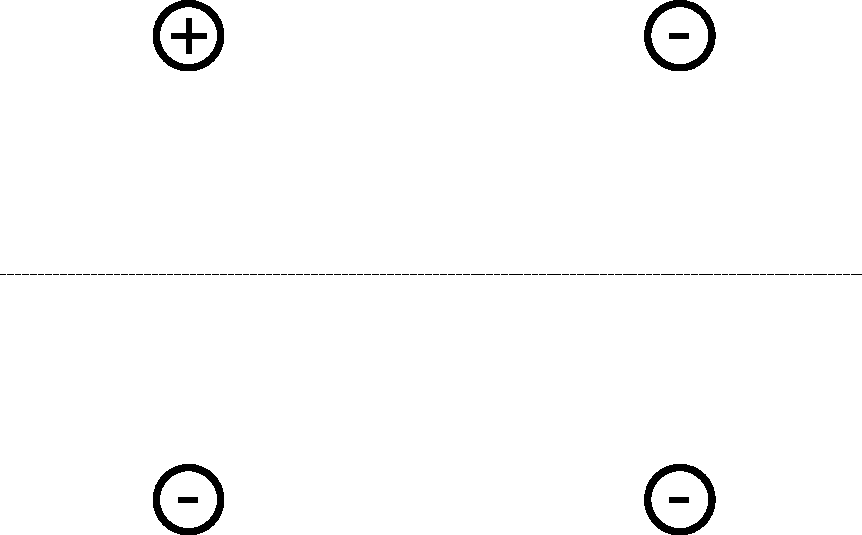
\includegraphics[width=0.6\textwidth]{images/two-pairs-charges.pdf}
	\end{centerinpage}
	%

%%%%%%%%%%%%%%%%%%%%%%%%%%%%%%%%%%%%%%%%%%%%%%%%%%%%
\newpage
	
	\item {\bf Electric Field} Physicists decided that they did not like ``instantaneous action at a distance'' forces,  so they introduce a new concept called the {\em Electric Field}.  Each charge produces its own electric field everywhere in space (with changes to the field, induced by motion of the charges, propagating outward at the speed of light). Then another charge can sit in the field of the first charge and experience a force due to the field (see next question).  
	
	For a positive charge, the electric field points outward in all directions, and is drawn as equally spaced lines emanating outward with arrowheads in the middle of thoses lines (not at the ends like an arrow/vector).  Negative charges have fields that look the same, but the arrowheads point inward.  Once you draw that field, you could go to any point in space, draw a dot, and draw {\em the electric field vector} at that point, $\vec{E}$, which is a vector/arrow that is parallel to the field lines at that point.  Draw the electric field lines in each of the two pictures shown below.  Make few points in space, and draw the electric field vectors at those points (these will be larger/stronger closer to the source charge).\\[72pt]
	%
	\begin{centerinpage}
	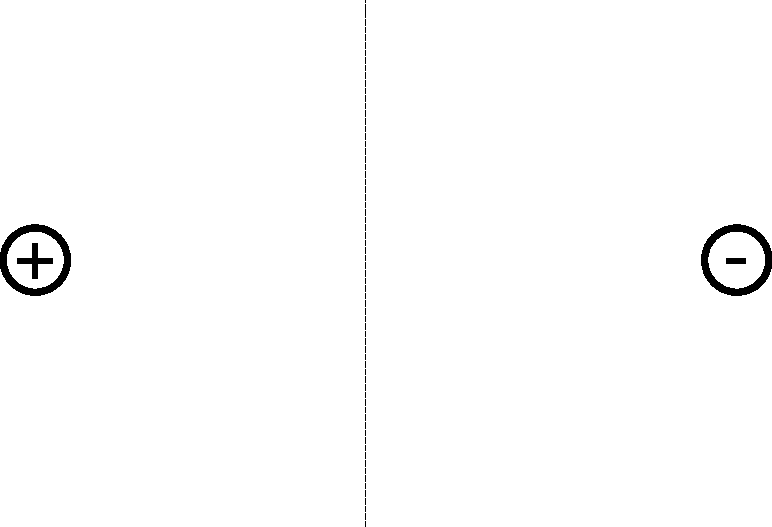
\includegraphics[width=0.7\textwidth]{images/two-charges-for-fields.pdf}
	\end{centerinpage}
	%

%%%%%%%%%%%%%%%%%%%%%%%%%%%%%%%%%%%%%%%%%%%%%%%%%%%%
\newpage

	\item {\bf Electric Field Force} The electric force law is given as $\vec{F}_{E \text{ on } q} = q \vec{E}$. This means that the force vector on a charge will {\em point the same direction as the field when the charge is positive}, but {\em the opposite direction when the charage is negative}. 
	
	Now consider the again the two pictures of charge pairs  (reproduced below).  In each picture, draw: (i) the field of the left charge ($q_1$) everywhere in the picture; (ii)  the electric field vector, $\vec{E}_1$, at the position  of the second charge; (iii) The force vector on the second charge, $\vec{F}_{E_1 \text{ on } q_2}$.\\[72pt]
	%
	\begin{centerinpage}
	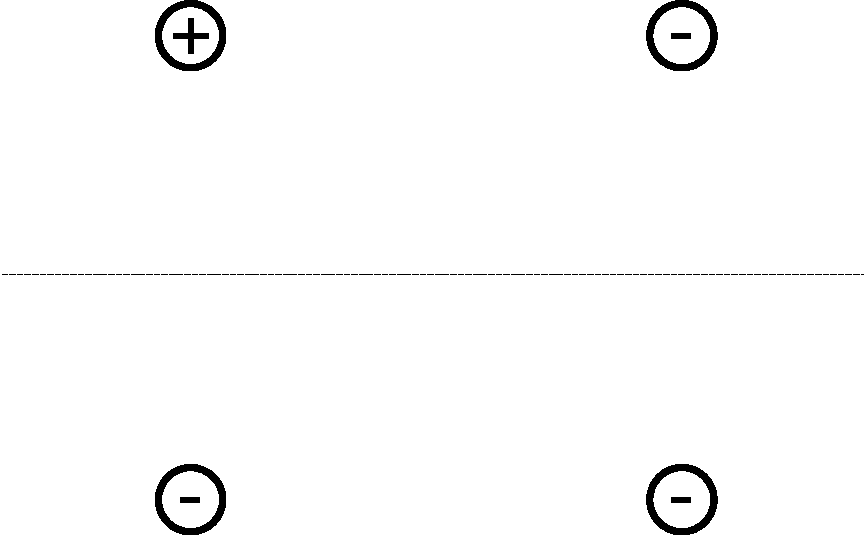
\includegraphics[width=0.7\textwidth]{images/two-pairs-charges_crop}
	\end{centerinpage}
	
%%%%%%%%%%%%%%%%%%%%%%%%%%%%%%%%%%%%%%%%%%%%%%%%%%%%
\newpage

	\item Now that we have the electric field, we can draw it and consider its effect on charges without considering the source charges that produced it.  Consider the {\em uniform} electric field below (same magnitude of $\vec{E}$ everywhere).   Draw a few little positive and negative charges in the field.  Indicate the $\vec{E}$ vector at their location.  And then draw the $\vec{F}_{E \text{ on } q}$ force vector on each charge. \\[72pt]
	%
	\begin{centerinpage}
	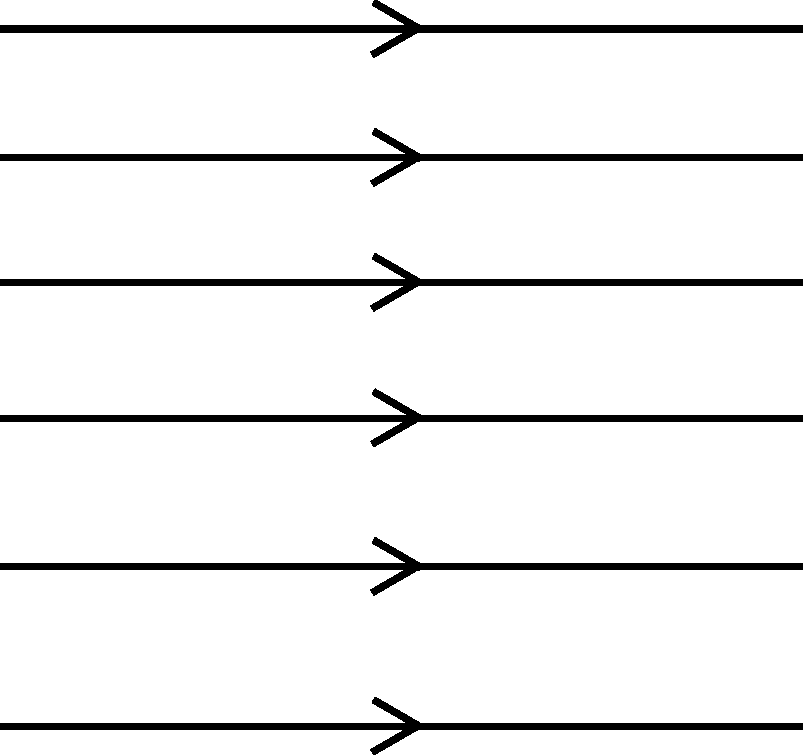
\includegraphics[width=\textwidth]{images/uniform-E-field}
	\end{centerinpage}

	
%%%%%%%%%%%%%%%%%%%%%%%%%%%%%%%%%%%%%%%%%%%%%%%%%%%%
\newpage
	
	\item {\bf Electric Dipole} An electric dipole can be thought of as: two opposite charges, $q$ and $-q$, separated by a rigid spring (with relaxed length, $d$).  Fill the space below with a uniform electric field (like the previous page)  and then draw multiple dipoles oriented in various orientations with respect to the field.  Indicate the force on each charge in the dipole. Describe the motion induced by the forces, if any\footnote{Remember, forces cause {\em accelerations}, meaning {\em changes in velocity}.  So if a dipole is placed in a field at rest, forces could cause it to {\em start moving} --- from zero velocity to some velocity.}

\vspace{10cm}

\noindent We represent an electric dipole schematically as a single vector, $\vec{\mu}$, that points from the positive to the negative charge, whose magnitude (strength) is $| \vec{\mu}| = |q| d$.  The sum of multiple dipoles creates a {\em net electric dipole}, and is found by {\bf vector addition}. Consider the ``tail to tip'' addition method shown at left and then try it for the other cases. \\[12pt]
	%
	\begin{centerinpage}
	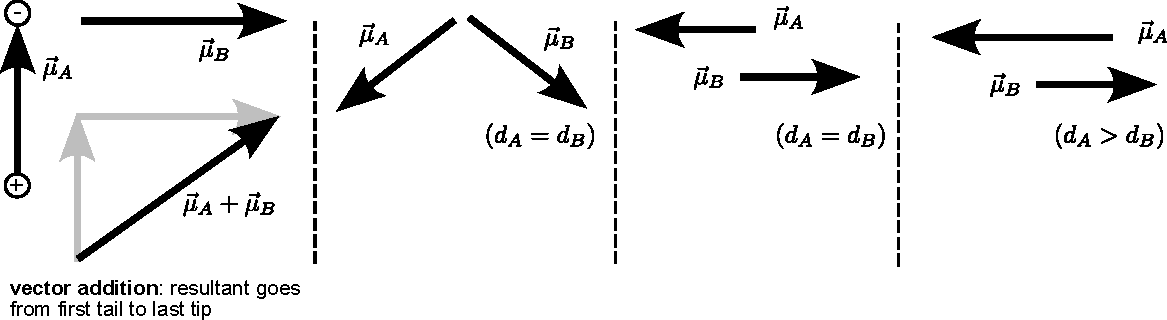
\includegraphics[width=\textwidth]{images/dipole-vector-addition}
	\end{centerinpage}


%%%%%%%%%%%%%%%%%%%%%%%%%%%%%%%%%%%%%%%%%%%%%%%%%%%%
\newpage
	
	\item {\bf Electromagnetic Waves}  To represent an electromagnetic (EM) wave traveling across the page from left to right: (i) draw an $x$-$y$ axis, with origin at left (long $x$ axis, short $y$); (ii) draw a sinusoidal wave along the $x$ axis [$y(x) = A \sin(x)$, so half in positive $y$, half in negative] with about three wavelengths spread across the page (show the length, $\lambda$), (iii) draw a velocity vector anywhere near the wave, labeled $\vec{v}$, pointing to the right.
	
	\vspace{4cm}
	
	\noindent Light is an {\em electromagnetic wave} and the $y$ direction of the wave you drew is meant to represent the {\em electric field} magnitude and direction (we will ignore the magnetic field part of the EM wave).\\[-6pt]
	
	\noindent \underline{Add the electric field to the picture above}: (iv) In between the $x$ axis and the sine curve, draw vertical electric field vectors with their tails on the axis. They point in the positive $y$ direction when the curve is positive, and in the negative direction when the curve is negative. The vectors have zero length twice per wavelength. This represents a {\em plane wave} of light, so the electric field vector at one position on the $x$ axis actually represents the electric field at all locations on an (infinite) 2D plane perpendicular to the axis there. \\[-6pt]
	
	\noindent \underline{In the space below}: (v) Using your plane wave above, now draw an electric field that fills the space. Use many $\vec{E}$ vectors (not ``field lines'' like prior questions).  Along any vertical line you should have multiple $\vec{E}$ vectors of the same length. (vi) Draw some electric dipoles,  sitting in this field and indicate the forces on their pairs of charges.

	\vspace{4cm}

	\noindent \underline{(vii) Look up the size of a few molecules listed on the first page.} We found earlier that the wavelength of infrared light is about one to 10 micrometers ($\unit{1}{\micro\meter}  = \unit{10^{-6}}{\meter}$).  How do these two sizes compare?  As an EM wave passes by a molecule, is there a lot of variation of the $\vec{E}$ field strength across the molecule, or a little? 

	\end{enumerate}
	
\newpage
%%%%%%%%%%%%%%%%%%%%%%%%%%%%%%%%%%%%%%%%%%%%%%%%%%
%%%%%%%%%%%      Chemistry atoms, molecules, geometry     %%%%%%%%%%%%%%%%
%%%%%%%%%%%%%%%%%%%%%%%%%%%%%%%%%%%%%%%%%%%%%%%%%%
\item {\bf Chemistry: Atoms, Molecules, Geometry, Dipoles}\\[-6pt]
	
Undergraduate physics majors take a course in Quantum Mechanics that culminates in constructing the discrete energy levels of a hydrogen atom, i.e., the possible excitations of a single electron bound to a single proton.  These energy levels are labeled by nested integers\footnote{The physical meaning of these labels correspond, approximately, to breaking the electron's three-dimensional motion around the proton into radial movement ($n$), and angular movement ($\ell$, $m$). The fourth label, $m_s$ corresponds to the ``spin'' of the electron.}
		%
		\begin{equation*}
		\begin{split}
		n &= 1, 2, 3, \ldots  \\
		 & \quad \ell = 0, 1, 2, \ldots, n-1 \\
		 & \quad \quad m = -\ell, -\ell + 1, \ldots, 0, \ldots, \ell - 1, \ell\\
		 & \quad \quad \quad m_s = -1, +1
		\end{split}
		\end{equation*}
		%
	where each energy level has a unique set of $(n, \ell, m, m_s)$, i.e., you choose one number from each row above.  For example, when hydrogen's electron is in the ``ground state'' (lowest energy level), it has $n=1$.  This means that $\ell = 0$ (since $\ell$ only goes up to $n-1$), which means that $m=0$ (since $m$ only goes up to $\pm \ell$), and then $m_s$ can be either $\pm 1$.  So the ground state of hydrogen is $(n, \ell, m, m_s) = (1, 0, 0, -1)$. 
	
	  It turns out that other atoms can be approximately constructed by ``filling'' the energy levels of hydrogen --- called the {\em orbitals} of hydrogen --- with additional electrons (and increasing the protons in the nucleus by the same number\footnote{Neutrons, the other particle in the nucleus of an atom, come along as well, with their number dictating the atomic mass.  An atom is defined by the number of protons (or electrons); changing the number of neutrons in an atom just changes the ``isotope.''  Atoms naturally occur with different numbers of neutrons. The atomic mass listed on the periodic table is an average over their frequency, which is dictated by the rules of nuclear physics and stability.}).  So, hydrogen with one electron fills the  $(1, 0, 0, -1)$ level, but helium has two electrons and fills two levels $(1, 0, 0, -1)$ and $(1, 0, 0, +1)$.  These are the only two levels with $n=1$, so the three-electron atom, lithium, fills the two levels of helium plus the level $(n, \ell, m, m_s) = (2, 0, 0, -1)$. 


	  
	  Chemistry uses this orbital model to build molecules\footnote{Here, we will consider only {\em covalent bonding}, where electrons are shared between neutral atoms.  Another type of bond, an {\em ionic bond},  is formed by the attractive electric force of positive and negative {\em ionized atoms} (atoms that have lost or gained one or more electrons, e.g., salt: $\text{Na}^+$ plus $\text{Cl}^-$ equals NaCl).} from atoms.  The first two rows of the periodic table (see next page) correspond to complete the $n=1$ and $n=2$ levels, respectively, and the third row corresponds to $n=3$ with $\ell = 0, 1$ ($\ell = 2$ appears on the fourth row, and we will ignore for now).  Each of these rows is considered a ``shell'' which is ``closed'' by reaching the end of a row.  The electrons in the ``outermost shell'' are called {\em valence} electrons.  The first row of the period table has up to two valence electrons, while the second and third rows have up to eight valence electrons (corresponding to the eight possible $\ell$ and $m$ values).   Molecules are formed following these rules (see also the figures on the next page):
		%
		\begin{itemize}
		\item Electrons are placed on atoms in a {\em Lewis dot} convention, with four pairs in the four cardinal directions (N, S, E, W). For H and He (the first row,  $n=1$, case), one pair.
		\item As the valence electrons are filled up (moving across a row in the periodic table), each pair receives one electron first, before pairs are filled with two electrons.		
		\item If two or more atoms form a molecule, each atom will ``fill'' its valence shell (obtain eight electrons), 
		\end{itemize}
	

	%
	\begin{enumerate}
	\item Form molecules for: $\text{N}_2$, $\text{O}_2$, $\text{C}\text{H}_4$, $\text{C}\text{O}_2$, and $\text{H}_2\text{O}$.  Use the rules described above and take these steps:
		%
		\begin{itemize}
		\item Draw the Lewis dot structure for each atom that will join to form the molecule first.
		\item Arrange the atoms next to each other so that unpaired electrons can be shared by neighboring atoms.
		\item Replace any shared pair of electrons with a solid line, leaving each atoms own pairs as two dots.
		\end{itemize}
		%
	\item Use the potatoes provided to physically build these molecules following your construction in the previous question.  Use big yellow potatoes for O, N, C, and little yellow potatoes for H.  Use little red potatoes for bonds and free electron pairs.  Hold everything together with sticks.  Try to arrange these such that the red potatoes are pushed furthest apart (this is the electric force repulsion of electrons).
	\item Given your physical structures, determine why the molecular structure of the greenhouse gas molecules are as described on the first page.
	\end{enumerate}

\newpage

\begin{center}
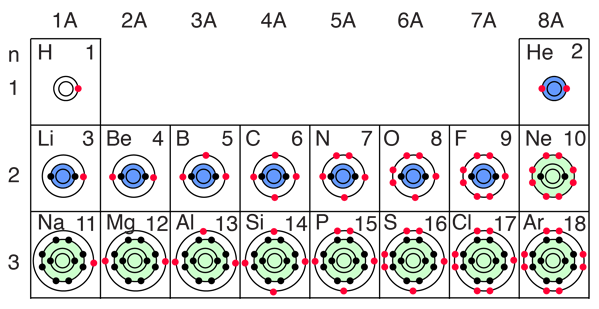
\includegraphics[width=0.38\textwidth]{images/atomic-orbitals-periodic-table_hyperphys_noalpha.png} %
\hfill %
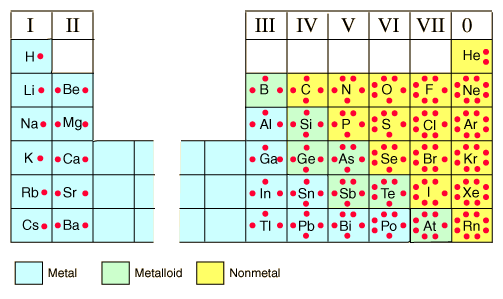
\includegraphics[width=0.55\textwidth]{images/lewis-dot-periodic-table_hyperphys.png}
\end{center}

\vspace{1cm}

%
\renewcommand{\arraystretch}{1.4}
\begin{center}
\begin{tabular}{|l|c|l|l|}
\hline
{\bf Atom}  & $N_{e^-} = N_p$ & {\bf Energy levels filled} \hspace{1cm} & {\bf ``Electron Configuration''} \hspace {0.5cm} \\
\hline
\hline
H & 1 & (1, 0, 0, -1) & $1 \text{s}^1$\\
\hline
He & 2 & (1, 0, 0, -1),  (1, 0, 0, +1) & $1 \text{s}^2$\\
\hline
\hline
Li & 3 & He + (2, 0, 0, -1) & $1 \text{s}^2  \, 2 \text{s}^1$\\
\hline
Be & 4 & Li + (2, 0, 0, +1) & $1 \text{s}^2 \, 2 \text{s}^2$\\
\hline
B & 5 & Be + (2, 1, -1, -1) & $1 \text{s}^2 \, 2 \text{s}^2 \, 2 \text{p}^1$\\
\hline
C & 6 & B + (2, 1, 0, -1) & $1 \text{s}^2 \, 2 \text{s}^2 \, 2 \text{p}^2$\\
\hline
N &7 & C + (2, 1, +1, -1) & $1 \text{s}^2 \, 2 \text{s}^2 \, 2 \text{p}^3$\\
\hline
O & 8 & N + (2, 1, -1, +1) & $1 \text{s}^2 \, 2 \text{s}^2 \, 2 \text{p}^4$\\
\hline
F & 9 & O + (2, 1, 0, +1) & $1 \text{s}^2 \, 2 \text{s}^2 \, 2 \text{p}^5$\\
\hline
Ne & 10 & F + (2, 1, +1, +1) & $1 \text{s}^2 \, 2 \text{s}^2 \, 2 \text{p}^6$\\
\hline
\hline
Na & 11 & Ne + (3, 0, 0, -1) & $1 \text{s}^2 \, 2 \text{s}^2 \, 2 \text{p}^6 \, 3\text{s}^1$ \\
\hline
Mg & 12 & Na + (3, 0, 0, +1) & $1 \text{s}^2 \, 2 \text{s}^2 \, 2 \text{p}^6 \, 3\text{s}^2$ \\
\hline
Al & 13 & Mg + (3, 1, -1, -1) & $1 \text{s}^2 \, 2 \text{s}^2 \, 2 \text{p}^1\, 3\text{s}^2 \, 3\text{p}^1$ \\
\hline
Si & 14 & Al + (3, 1, 0, -1) & $1 \text{s}^2 \, 2 \text{s}^2 \, 2 \text{p}^2\, 3\text{s}^2 \, 3\text{p}^2$ \\
\hline
P & 15 & Si + (3, 1, +1, -1) & $1 \text{s}^2 \, 2 \text{s}^2 \, 2 \text{p}^3 \, 3\text{s}^2 \, 3\text{p}^3$ \\
\hline
S & 16 & P + (3, 1, -1, +1) & $1 \text{s}^2 \, 2 \text{s}^2 \, 2 \text{p}^4 \, 3\text{s}^2 \, 3\text{p}^4$ \\
\hline
Cl & 17 & S  + (3, 1, 0, +1) & $1 \text{s}^2 \, 2 \text{s}^2 \, 2 \text{p}^5 \, 3\text{s}^2 \, 3\text{p}^5$ \\
\hline
Ar & 18 & Cl + (3, 1, +1, +1) & $1 \text{s}^2 \, 2 \text{s}^2 \, 2 \text{p}^6 \, 3\text{s}^2 \, 3\text{p}^6$ \\
\hline
\end{tabular}
\end{center}


\newpage
%%%%%%%%%%%%%%%%%%%%%%%%%%%%%%%%%%%%%%%%%%%%%%%%%%
%%%%%%%%%%%      Chemistry atoms, molecules, geometry     %%%%%%%%%%%%%%%%
%%%%%%%%%%%%%%%%%%%%%%%%%%%%%%%%%%%%%%%%%%%%%%%%%%
\item {\bf Interaction of Light with Molecules: Vibrational Modes,  Dipoles, Rotation}
	%
	\begin{enumerate}
	\item Assign a dipole vector to each red potato on your physical models (or if less daring, just try to draw on your written models).  
	\item Imagine possible rotations and vibrations of each molecule and try to understand:
		%
		\begin{enumerate}
		\item Why are water, methane, and carbon dioxide greenhouse gases?  
		\item Why are oxygen and nitrogen not greenhouse gases?
		\end{enumerate}
	\end{enumerate}



\end{enumerate}
	
%%%%%%%%%%%%%%%%%%%%%%%%%%%%%%%%%%%%%%%%%%%%%%%%
%%%%%%%%%%%%%      astronomical info           %%%%%%%%%%%%%%%%%%%%%
%%%%%%%%%%%%%%%%%%%%%%%%%%%%%%%%%%%%%%%%%%%%%%%%


%\newpage
%\thispagestyle{empty}
%\mbox{}

%\newpage
%%%%%%%%%%%%%%%%%%%%%%%%%%%%%%%%%%%%%%%%%%%%%%%%%%%%
%%%%%%%%%%                           Extras                           %%%%%%%%%%%%%%
%%%%%%%%%%%%%%%%%%%%%%%%%%%%%%%%%%%%%%%%%%%%%%%%%%%%




%%%%%%%%%%%%%%%%%%%%%%%%%%%%%%%%%%%%%%%%%%%%%%%%%%%%
%%%%%%%%%%                                  References                                %%%%%%%%%%%%%%%%
%%%%%%%%%%%%%%%%%%%%%%%%%%%%%%%%%%%%%%%%%%%%%%%%%%%%
%\noindent {\bf Data Sources}: 



\end{document}
